\documentclass[11pt]{article}
% ===========================================================================
%  Shared preamble for all MDM4U worksheets — input right after \documentclass.
%  (Files beginning with "_" are skipped by mdm4u-worksheet-publish.mjs.)
% ===========================================================================
\usepackage[letterpaper,top=2.2cm,bottom=1.9cm,left=1.6cm,right=1.6cm,headheight=28pt,footskip=24pt]{geometry}
\usepackage{amsmath,amssymb}
\usepackage[T1]{fontenc}
\usepackage[utf8]{inputenc}
\usepackage{lmodern}
\usepackage{xcolor}
\usepackage[most]{tcolorbox}
\usepackage{enumitem}
\usepackage{multicol}
\usepackage{fancyhdr}
\usepackage{array}
\usepackage{tikz}
\usetikzlibrary{calc}
\usepackage{pgfplots}
\pgfplotsset{compat=1.18}

\definecolor{exblue}{HTML}{4A90E2}
\definecolor{exbg}{HTML}{E6F3FF}
\definecolor{qorange}{HTML}{E69138}
\definecolor{qbg}{HTML}{FFF7CC}
\definecolor{keygray}{HTML}{475569}
\definecolor{keybg}{HTML}{F1F5F9}
\definecolor{iagreen}{HTML}{14653B}
\definecolor{titleblue}{HTML}{1D4ED8}
% Rotating palette so each worked example gets its own colour.
\definecolor{ex0}{HTML}{2563A0}\definecolor{ex1}{HTML}{3B7D3B}\definecolor{ex2}{HTML}{8A5A00}
\definecolor{ex3}{HTML}{A3327A}\definecolor{ex4}{HTML}{6D28A3}\definecolor{ex5}{HTML}{B08900}
\definecolor{ex6}{HTML}{0E7490}\definecolor{ex7}{HTML}{9A3412}\definecolor{ex8}{HTML}{15803D}

\pagestyle{fancy}
\fancyhf{}
\fancyhead[L]{\footnotesize NAME: \underline{\hspace{3.4cm}}}
\fancyhead[C]{\textbf{Integration Academy}\\[-2pt]{\scriptsize Math Simplified \textperiodcentered{} Success Amplified}}
\fancyhead[R]{\footnotesize MDM4U}
\fancyfoot[L]{\scriptsize dr.merie@IntegrationAcademy.ca}
\fancyfoot[C]{\scriptsize\thepage}
\fancyfoot[R]{\scriptsize IntegrationAcademy.ca}
\renewcommand{\headrulewidth}{1.2pt}
\renewcommand{\footrulewidth}{0.4pt}
\setlength{\parindent}{0pt}
\setlength{\parskip}{4pt}

% Examples are NOT breakable, so each example + its solution stays on one page.
\newtcolorbox{example}[2]{colframe=#1,colback=#1!7,coltitle=white,colbacktitle=#1,fonttitle=\bfseries,title={#2},arc=3pt,boxrule=1pt}
\newtcolorbox{qbox}[1]{colframe=qorange,colback=qbg,coltitle=white,colbacktitle=qorange,fonttitle=\bfseries,title={#1},arc=3pt,breakable,boxrule=1pt}
\newtcolorbox{keybox}{colframe=keygray,colback=keybg,coltitle=white,colbacktitle=keygray,fonttitle=\bfseries,title={$\checkmark$\ Answer Key},arc=3pt,breakable,boxrule=1pt}
\newtcolorbox{recapbox}{colframe=keygray,colback=keybg,coltitle=white,colbacktitle=keygray,fonttitle=\bfseries,title={Question Recap},arc=3pt,breakable,boxrule=1pt}
\newtcolorbox{ideabox}{colframe=titleblue,colback=titleblue!6,coltitle=white,colbacktitle=titleblue,fonttitle=\bfseries,title={The Big Ideas},arc=3pt,breakable,boxrule=1.2pt}
\newtcolorbox{learnbox}{colframe=iagreen,colback=iagreen!5,coltitle=white,colbacktitle=iagreen,fonttitle=\bfseries,title={Concept in Focus},arc=3pt,breakable,boxrule=1.2pt}
\newcommand{\lh}[1]{\par\smallskip{\bfseries\color{iagreen}#1}\par\nobreak\smallskip}

\newcommand{\soln}{\par\smallskip\textit{\textbf{Solution.}}\ }
\newcommand{\workspace}[1]{\par\vspace{3pt}\fcolorbox{black!30}{white}{\begin{minipage}[t][#1][t]{\dimexpr\linewidth-2\fboxsep\relax}\ \end{minipage}}\par}
\newcommand{\sech}[1]{\par\vspace{8pt}{\Large\bfseries\color{iagreen}#1}\par\nobreak\vspace{2pt}{\color{black!20}\hrule height1pt}\vspace{6pt}}

% A compact coordinate plot sized for an example box: \eplot{xmin}{xmax}{ymin}{ymax}{body}
\newcommand{\eplot}[5]{\begin{center}\begin{tikzpicture}
\begin{axis}[width=6.8cm,height=4.4cm,axis lines=middle,xlabel={\tiny$x$},ylabel={\tiny$y$},
grid=both,grid style={gray!16},xmin=#1,xmax=#2,ymin=#3,ymax=#4,
xtick distance=2,ytick distance=2,tick label style={font=\tiny},axis line style={-},samples=120]
#5
\end{axis}\end{tikzpicture}\end{center}}

% Standard-normal bell with a shaded region between #1 and #2 (in z): \ncurve{from}{to}{extra body}
\newcommand{\ncurve}[3]{\begin{center}\begin{tikzpicture}
\begin{axis}[width=8.6cm,height=4.2cm,axis lines=middle,xlabel={\tiny$z$},ylabel={},
xmin=-3.8,xmax=3.8,ymin=0,ymax=0.45,xtick={-3,-2,-1,0,1,2,3},ytick=\empty,
tick label style={font=\tiny},axis line style={-},samples=160,domain=-3.8:3.8]
\addplot[exblue,very thick]{1/sqrt(2*pi)*exp(-x^2/2)};
\addplot[exblue!22,fill=exblue!22,domain=#1:#2]{1/sqrt(2*pi)*exp(-x^2/2)}\closedcycle;
#3
\end{axis}\end{tikzpicture}\end{center}}

% A bar chart / histogram from (x,height) coordinates: \hist{ymax}{coords}
\newcommand{\hist}[2]{\begin{center}\begin{tikzpicture}
\begin{axis}[width=8.6cm,height=4.6cm,axis lines=left,ybar,bar width=13pt,
ymin=0,ymax=#2, enlarge x limits=0.12,grid=both,grid style={gray!14},
tick label style={font=\tiny},axis line style={-}]
\addplot[draw=exblue,fill=exbg] coordinates {#1};
\end{axis}\end{tikzpicture}\end{center}}

% A box-and-whisker plot on a number line: \boxplot{min}{Q1}{med}{Q3}{max}{axmin}{axmax}
\newcommand{\boxplot}[7]{\begin{center}\begin{tikzpicture}[yscale=0.5]
\draw[gray!40] (#6,0)--(#7,0);
\foreach \t in {#6,...,#7}{\draw[gray!40] (\t,-0.12)--(\t,0.12) node[below=2pt,font=\tiny]{\t};}
\draw[exblue,very thick] (#2,-0.7) rectangle (#4,0.7);
\draw[qorange,very thick] (#3,-0.7)--(#3,0.7);
\draw[exblue,thick] (#1,0)--(#2,0);\draw[exblue,thick] (#4,0)--(#5,0);
\draw[exblue,thick] (#1,-0.4)--(#1,0.4);\draw[exblue,thick] (#5,-0.4)--(#5,0.4);
\end{tikzpicture}\end{center}}

% A scatter plot: \scatter{xmin}{xmax}{ymin}{ymax}{body}
\newcommand{\scatter}[5]{\begin{center}\begin{tikzpicture}
\begin{axis}[width=7.6cm,height=5cm,axis lines=middle,xlabel={\tiny$x$},ylabel={\tiny$y$},
grid=both,grid style={gray!16},xmin=#1,xmax=#2,ymin=#3,ymax=#4,
tick label style={font=\tiny},axis line style={-}]
#5
\end{axis}\end{tikzpicture}\end{center}}

% A labelled scatter plot: \scatterl{xmin}{xmax}{ymin}{ymax}{xlabel}{ylabel}{body}
\newcommand{\scatterl}[7]{\begin{center}\begin{tikzpicture}
\begin{axis}[width=8.6cm,height=5.4cm,axis lines=left,xlabel={\small #5},ylabel={\small #6},
grid=both,grid style={gray!16},xmin=#1,xmax=#2,ymin=#3,ymax=#4,
tick label style={font=\scriptsize},axis line style={-}]
#7
\end{axis}\end{tikzpicture}\end{center}}

\fancyhead[R]{\footnotesize MDM4U \textperiodcentered{} 6.1}
\begin{document}

\begin{center}
{\LARGE\bfseries\color{titleblue}Worksheet 6.1 --- Scatter Plots \& Correlation}\\[2pt]
{\small Grade 12 Mathematics of Data Management (MDM4U) \textperiodcentered{} Unit 6: Two-Variable Statistics}
\end{center}

\begin{ideabox}
A scatter plot shows paired data as points. Describe it by \emph{direction}, \emph{form}, \emph{strength} and \emph{unusual features}, in context. The correlation coefficient $r$ (from technology) measures the strength and direction of a \emph{linear} relationship, from $-1$ to $1$. A strong correlation shows \emph{association}, not necessarily \emph{cause and effect}.
\begin{itemize}[leftmargin=*,itemsep=2pt]
  \item Explanatory ($x$) variable predicts; response ($y$) variable is predicted. Roles are not a claim of cause.
  \item Describe: direction (positive/negative), form (linear/curved), strength, unusual features (outliers, clusters).
  \item $-1\le r\le1$: sign $=$ direction, $|r|=$ strength, $r$ detects only \emph{linear} association, and one outlier can change it a lot.
  \item $r$ has no units; changing units or swapping axes keeps $r$; reversing one scale flips its sign.
  \item Correlation $\ne$ causation. Name the type of relationship: cause and effect, common cause, reverse cause and effect, presumed, or accidental --- and justify it with the reason for the link.
\end{itemize}
\end{ideabox}

\begin{learnbox}
\lh{Two variables at once}A \textbf{scatter plot} graphs \emph{paired data}, one point per individual. The \textbf{explanatory} variable ($x$) is used to predict the \textbf{response} variable ($y$); label both axes with names and units.
\lh{Describe every scatter in four parts}\textbf{Direction} (positive or negative), \textbf{form} (linear or curved), \textbf{strength} (how tightly the points follow the pattern) and \textbf{unusual features} (outliers, separate clusters) --- always in the context of the problem.
\lh{The correlation coefficient $r$}Technology gives $r$, with $-1\le r\le1$. The sign is the direction and $|r|$ the strength (about $0.8$ or more is strong). It measures only \emph{linear} association, has no units, and a single outlier can change it a lot. $r\approx0$ means no \emph{linear} relationship, not no relationship.
\lh{Five types of relationship}A strong correlation shows \textbf{association}, not cause. Classify it as \textbf{cause and effect} (a change in $x$ directly causes a change in $y$), \textbf{common cause} (a third variable drives both), \textbf{reverse cause and effect} (the roles are backwards), \textbf{presumed} (sensible link, but no cause or third variable can be named) or \textbf{accidental} (coincidence). Justify the type with the reason for the link; a \textbf{randomized experiment} gives the strongest support for cause and effect.
\end{learnbox}

\sech{Worked Examples}

\begin{example}{ex0}{Example 1 --- Assign the roles}
Name the explanatory and response variable. \\ \textbf{(a)} A teen's nightly sleep and next-day reaction time. \\ \textbf{(b)} A tree's age and its trunk diameter. \\ \textbf{(c)} A company's monthly advertising spending and its website visits.\soln (a) explanatory: hours of sleep; response: reaction time. (b) explanatory: age; response: trunk diameter. (c) explanatory: advertising spending; response: website visits. In each case the first variable is the one used to predict the second.
\end{example}

\begin{example}{ex1}{Example 2 --- Plot and describe}
The age of nine used cars and their resale value are recorded. Technology gives $r=-0.998$. Describe the relationship.\begin{center}\footnotesize\begin{tabular}{|l|*{9}{c|}}\hline Age (years) & 1 & 2 & 3 & 4 & 5 & 6 & 7 & 8 & 9 \\ \hline Value (\$1000s) & 24.1 & 21.2 & 19.8 & 17.9 & 15.3 & 13.6 & 11.2 & 9.8 & 8.1 \\ \hline\end{tabular}\end{center}\scatterl{0}{10}{0}{26}{Age of car (years)}{Value (\$1000s)}{\addplot[only marks,mark=*,exblue,mark size=2pt] coordinates {(1,24.1)(2,21.2)(3,19.8)(4,17.9)(5,15.3)(6,13.6)(7,11.2)(8,9.8)(9,8.1)};}\soln The points fall steadily from upper left to lower right and hug a straight band: a \textbf{strong, negative, linear} relationship between a car's age and its resale value, with no unusual features.
\end{example}

\begin{example}{ex2}{Example 3 --- A weak relationship}
Ten adults record their average daily steps (in thousands) and their resting heart rate. Technology gives $r=-0.37$. Describe the relationship.\begin{center}\footnotesize\begin{tabular}{|l|*{10}{c|}}\hline Steps (1000s) & 3 & 4 & 5 & 6 & 7 & 8 & 9 & 10 & 11 & 12 \\ \hline Heart rate (bpm) & 72 & 76 & 69 & 75 & 70 & 73 & 68 & 74 & 71 & 69 \\ \hline\end{tabular}\end{center}\scatterl{2}{13}{64}{80}{Daily steps (thousands)}{Resting heart rate (bpm)}{\addplot[only marks,mark=*,exblue,mark size=2pt] coordinates {(3,72)(4,76)(5,69)(6,75)(7,70)(8,73)(9,68)(10,74)(11,71)(12,69)};}\soln There is a slight downward drift (\textbf{negative}), the points are loosely scattered about a line (\textbf{linear}, but \textbf{weak}, $|r|=0.37$): more steps goes with a slightly lower heart rate, but individual points vary widely. No outliers.
\end{example}

\begin{example}{ex3}{Example 4 --- A pattern that $r$ misses}
A ball's height is recorded each second after it is thrown. Technology gives $r=0$. Is height unrelated to time?\begin{center}\footnotesize\begin{tabular}{|l|*{7}{c|}}\hline Time (s) & 0 & 1 & 2 & 3 & 4 & 5 & 6 \\ \hline Height (m) & 1 & 6 & 9 & 10 & 9 & 6 & 1 \\ \hline\end{tabular}\end{center}\scatterl{-0.5}{6.5}{0}{12}{Time (s)}{Height (m)}{\addplot[only marks,mark=*,exblue,mark size=2pt] coordinates {(0,1)(1,6)(2,9)(3,10)(4,9)(5,6)(6,1)};}\soln No. The points trace a clear symmetric arch, so the relationship is strong but \textbf{non-linear}: it rises, then falls, so there is no overall direction. $r=0$ only says there is no \emph{linear} trend.
\end{example}

\begin{example}{ex4}{Example 5 --- An outlier from a recording error}
Heights of children aged 3 to 10 are entered in a spreadsheet; the age-8 height was typed as $12.7$ instead of $127$. Technology gives $r=0.12$ with the error and $r=0.998$ after correcting it.\begin{center}\footnotesize\begin{tabular}{|l|*{8}{c|}}\hline Age (years) & 3 & 4 & 5 & 6 & 7 & 8 & 9 & 10 \\ \hline Height (cm) & 96 & 103 & 110 & 116 & 122 & 12.7 & 133 & 138 \\ \hline\end{tabular}\end{center}\scatterl{2}{11}{0}{150}{Age (years)}{Height (cm)}{\addplot[only marks,mark=*,exblue,mark size=2pt] coordinates {(3,96)(4,103)(5,110)(6,116)(7,122)(9,133)(10,138)};\addplot[only marks,mark=*,red,mark size=2.8pt] coordinates {(8,12.7)};}\soln The point $(8,12.7)$ is a far outlier that drags $r$ from $0.998$ to $0.12$, hiding a very strong, positive, linear relationship. Because the cause is a known typing error, \emph{correct} it to $127$ (and say so); do not simply delete points to improve $r$.
\end{example}

\begin{example}{ex5}{Example 6 --- Rank by strength}
For plants, technology gives $r$ between height after six weeks and: sunlight hours $0.88$; daily water $0.52$; soil pH $-0.12$; night temperature $-0.93$. Which has the strongest relationship, which the weakest, and which are negative?\soln Compare $|r|$: $0.93>0.88>0.52>0.12$. Strongest: night temperature ($-0.93$). Weakest: soil pH ($-0.12$). Negative: night temperature and soil pH.
\end{example}

\begin{example}{ex6}{Example 7 --- Units and reversed scales}
Distance run $x$ (km) and calories burned $y$ have $r=0.89$. Find $r$ if \\ \textbf{(a)} distance is in miles; \\ \textbf{(b)} the axes are swapped; \\ \textbf{(c)} $y$ is replaced by $1000-y$ (calories \emph{remaining} of a 1000 kcal goal).\soln (a) $0.89$ --- units do not change $r$. (b) $0.89$ --- $r$ is symmetric in $x$ and $y$. (c) $-0.89$ --- reversing one scale flips the sign only.
\end{example}

\begin{example}{ex7}{Example 8 --- Two hidden groups}
Shoe size and reading speed (words per minute) are recorded for Grade 2 students (blue) and Grade 8 students (orange). All 15 students give $r=0.96$; within Grade 2 alone $r=-0.18$; within Grade 8 alone $r=-0.05$.\scatterl{26}{45}{40}{170}{Shoe size (EU)}{Words per minute}{\addplot[only marks,mark=*,exblue,mark size=2pt] coordinates {(28,62)(29,70)(30,58)(31,66)(32,60)(29.5,64)(30.5,68)};\addplot[only marks,mark=*,qorange,mark size=2pt] coordinates {(38,150)(39,142)(40,158)(41,148)(42,155)(43,146)(39.5,152)(41.5,144)};}\soln The combined $r$ is strong only because of the \emph{gap between two clusters}. Inside each grade there is no linear pattern ($r$ near $0$). Grade level (age) is the hidden factor driving both shoe size and reading speed; do not describe the combined data as one linear trend.
\end{example}

\begin{example}{ex8}{Example 9 --- Name the type of relationship}
Each pair is positively correlated. Name the most likely type of relationship and justify it. \\ \textbf{(a)} The number of fire trucks sent to a fire and the dollar damage. \\ \textbf{(b)} The number of snowplows a city owns and its yearly snowfall. \\ \textbf{(c)} Hours of practice and a dancer's competition score. \\ \textbf{(d)} The number of vowels in a town's name and the town's population. \\ \textbf{(e)} A person's grip strength and their running speed.\soln (a) \emph{Common cause}: the size of the fire drives both. (b) \emph{Reverse cause and effect}: heavy snowfall leads a city to buy more plows. (c) \emph{Cause and effect}: practice directly improves skill (a clear mechanism, though a sample should be large). (d) \emph{Accidental}: no logical link. (e) \emph{Presumed}: both reflect general fitness, but neither causes the other and no single third variable is obvious.
\end{example}

\clearpage
\sech{Your Turn --- Show Your Work}
For each question, show all steps clearly in the space provided.

\begin{qbox}{Question 1}
Name the explanatory and response variables: a river's water level (m) and the day's rainfall (mm).\workspace{1.6cm}
\end{qbox}

\begin{qbox}{Question 2}
Eight musicians record weekly practice hours and the number of mistakes in a recital. Technology gives $r=-0.98$. Describe the relationship in context.\begin{center}\footnotesize\begin{tabular}{|l|*{8}{c|}}\hline Practice (h/week) & 1 & 2 & 3 & 4 & 5 & 6 & 7 & 8 \\ \hline Mistakes & 14 & 12 & 13 & 10 & 9 & 7 & 6 & 4 \\ \hline\end{tabular}\end{center}\scatterl{0}{9}{0}{16}{Practice (hours/week)}{Mistakes}{\addplot[only marks,mark=*,exblue,mark size=2pt] coordinates {(1,14)(2,12)(3,13)(4,10)(5,9)(6,7)(7,6)(8,4)};}\workspace{2.2cm}
\end{qbox}

\begin{qbox}{Question 3}
Match each value of $r$ to a description: $0.97,\ -0.33,\ 0.62,\ -0.91$. Descriptions: strong negative, weak negative, moderate positive, strong positive.\workspace{2.4cm}
\end{qbox}

\begin{qbox}{Question 4}
Name the most likely type of relationship and justify it. \\ \textbf{(a)} Umbrella sales and raincoat sales in a town. \\ \textbf{(b)} The number of passengers on a bus and the bus's total fuel use. \\ \textbf{(c)} The number of letters in a student's surname and their test score. \\ \textbf{(d)} A city's number of hospitals and its number of schools.\workspace{3.4cm}
\end{qbox}

\begin{qbox}{Question 5}
All points lie exactly on a straight line that rises to the right. What is $r$? What is $r$ if the line falls?\workspace{2cm}
\end{qbox}

\begin{qbox}{Question 6}
The data below follow $y=2^{x}$ and technology gives $r=0.88$. Describe the form, and explain why \textquotedblleft{}strong linear relationship\textquotedblright{} would be a poor description.\begin{center}\footnotesize\begin{tabular}{|l|*{7}{c|}}\hline $x$ & 0 & 1 & 2 & 3 & 4 & 5 & 6 \\ \hline $y$ & 1 & 2 & 4 & 8 & 16 & 32 & 64 \\ \hline\end{tabular}\end{center}\scatterl{-1}{7}{0}{70}{$x$}{$y$}{\addplot[only marks,mark=*,exblue,mark size=2pt] coordinates {(0,1)(1,2)(2,4)(3,8)(4,16)(5,32)(6,64)};}\workspace{2.2cm}
\end{qbox}

\begin{qbox}{Question 7}
A scatter plot has $r=-0.31$. After one far-off point is removed, $r=-0.94$. \\ \textbf{(a)} What does this show? \\ \textbf{(b)} What must you do before deleting the point?\workspace{2.6cm}
\end{qbox}

\begin{qbox}{Question 8}
A survey finds that adults who take a daily vitamin have lower blood pressure ($r=-0.40$). \\ \textbf{(a)} Give two explanations other than \textquotedblleft{}vitamins lower blood pressure\textquotedblright{}. \\ \textbf{(b)} Describe a study that could test whether vitamins really do lower blood pressure.\workspace{3.2cm}
\end{qbox}

\begin{qbox}{Question 9}
Countries with more televisions per person have longer life expectancy ($r=0.80$). Does owning televisions lengthen life? Name a lurking variable.\workspace{2.4cm}
\end{qbox}

\begin{qbox}{Question 10}
Streets with more security cameras report more break-ins ($r=0.60$). Explain how reverse cause could account for this.\workspace{2.4cm}
\end{qbox}

\begin{qbox}{Question 11}
Sketch a scatter plot of about eight points that is positive, linear and weak, with one outlier.
\begin{center}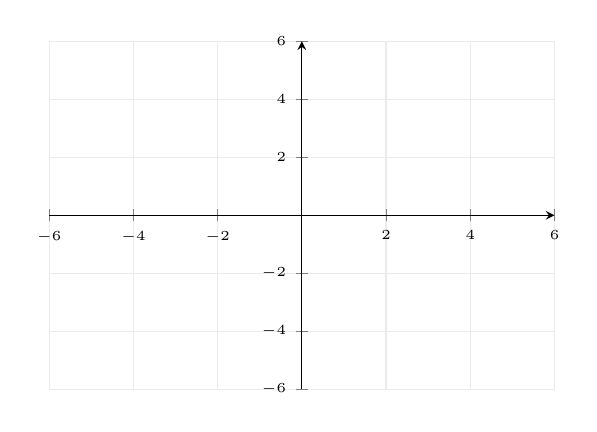
\begin{tikzpicture}\begin{axis}[width=8cm,height=6cm,axis lines=middle,grid=both,grid style={gray!16},xmin=-6,xmax=6,ymin=-6,ymax=6,xtick distance=2,ytick distance=2,tick label style={font=\tiny}]\end{axis}\end{tikzpicture}\end{center}
\end{qbox}

\begin{qbox}{Question 12}
A classmate says \textquotedblleft{}$r=0.92$ means 92\% of the points lie on the line.\textquotedblright{} Explain the error.\workspace{2.4cm}
\end{qbox}

\begin{qbox}{Question 13 --- Challenge}
A food truck records the day's high temperature and the cups of lemonade sold. Technology gives $r=0.99$.\begin{center}\footnotesize\begin{tabular}{|l|*{8}{c|}}\hline High ($^\circ$C) & 18 & 20 & 22 & 24 & 26 & 28 & 30 & 32 \\ \hline Cups sold & 41 & 49 & 48 & 58 & 62 & 66 & 74 & 79 \\ \hline\end{tabular}\end{center}\par\smallskip\textbf{(a)} Name the explanatory and response variables. \\ \textbf{(b)} Describe the relationship. \\ \textbf{(c)} Find $r$ if temperature is converted to $^\circ$F. \\ \textbf{(d)} A rainy day at $24^\circ$C sells only 12 cups. How would this point appear, and what would it do to $r$? \\ \textbf{(e)} Does hot weather \emph{cause} higher sales? What would you need to be sure?\workspace{6.5cm}
\end{qbox}

\clearpage
\sech{Question Recap \& Answer Key}

\begin{recapbox}
\begin{multicols}{2}
\small
\begin{enumerate}[leftmargin=*,itemsep=3pt]
  \item Name the explanatory and response variables: a river's water level (m) and the day's rainfall (mm).
  \item Describe the practice-vs-mistakes scatter plot ($r=-0.98$) in context.
  \item Match each value of $r$ to a description: $0.97,\ -0.33,\ 0.62,\ -0.91$. Descriptions: strong negative, weak negative, moderate positive, strong positive.
  \item Name the type of relationship (cause and effect, common cause, reverse, presumed or accidental) for four pairs.
  \item All points lie exactly on a straight line that rises to the right. What is $r$? What is $r$ if the line falls?
  \item Data follow $y=2^x$ ($r=0.88$): describe the form and say why \textquotedblleft{}strong linear\textquotedblright{} is a poor description.
  \item A scatter plot has $r=-0.31$. After one far-off point is removed, $r=-0.94$. \\ \textbf{(a)} What does this show? \\ \textbf{(b)} What must you do before deleting the point?
  \item Vitamins and blood pressure ($r=-0.40$): two other explanations; design a study to test cause.
  \item Countries with more televisions per person have longer life expectancy ($r=0.80$). Does owning televisions lengthen life? Name a lurking variable.
  \item Streets with more security cameras report more break-ins ($r=0.60$). Explain how reverse cause could account for this.
  \item Sketch a positive, linear, weak scatter with one outlier.
  \item A classmate says \textquotedblleft{}$r=0.92$ means 92\% of the points lie on the line.\textquotedblright{} Explain the error.
  \item Lemonade truck ($r=0.99$): (a) roles; (b) describe; (c) $^\circ$F; (d) effect of a 12-cup rainy day; (e) cause and effect?
\end{enumerate}
\end{multicols}
\end{recapbox}

\begin{keybox}
\begin{multicols}{2}
\small
\begin{enumerate}[leftmargin=*,itemsep=3pt]
  \item explanatory: rainfall; response: water level
  \item strong, negative, linear: more practice goes with fewer mistakes; no outliers
  \item $0.97$ strong positive; $-0.33$ weak negative; $0.62$ moderate positive; $-0.91$ strong negative
  \item (a) common cause (rainy weather); (b) cause and effect (more passengers weigh more, so more fuel); (c) accidental (no logical link); (d) common cause (city population)
  \item $r=1$ (rising line); $r=-1$ (falling line)
  \item curved (exponential growth) and increasing; $r$ measures only linear fit, so $0.88$ overstates a line's suitability
  \item (a) one outlier hid a strong negative linear pattern; (b) find out why it is unusual; correct or delete only if it is an error, otherwise keep it and report both $r$ values
  \item (a) common cause: people who take vitamins may exercise and eat better; reverse cause: people already watching their health are the ones who take vitamins; (b) randomly assign volunteers to a vitamin group or a placebo group, keep all else the same, and compare blood pressure
  \item no; lurking variable: national wealth/health care, which raises both
  \item crime leads residents to install cameras, so break-ins (the response) cause the cameras (the \textquotedblleft{}explanatory\textquotedblright{} variable)
  \item about eight points rising loosely, plus one point far from the pattern
  \item $r$ measures the strength of a \emph{linear} trend, not a percent of points; few points lie exactly on a line unless $|r|=1$
  \item (a) explanatory: temperature; response: cups sold; (b) strong, positive, linear; (c) $0.99$ (unchanged); (d) a point far below the pattern (outlier) that would lower $r$; (e) no; association only --- a randomized experiment would be needed
\end{enumerate}
\end{multicols}
\end{keybox}

\end{document}
